%-------------------------------------------------------------------------------
%                                PREAMBLE
%-------------------------------------------------------------------------------
\documentclass[usenames,dvipsnames,svgnames,10pt,aspectratio=169]{beamer}
\usefonttheme{professionalfonts}

% This theme uses TIKZ: compile twice with PDFLaTeX or LuaLaTeX.
%
%  Options:
%  - [clean]:    clean slides, i.e. logos and footbar are removed
%  - [kth]:      footbar style inspierd to the official KTH template
%  - [nicewave]: a different style of wave is used (not approved by FLOW)
%
\usetheme{flow}

\usepackage{hyperref,graphicx,lmodern}
\usepackage[utf8]{inputenc}
\usepackage{media9}
\usepackage{xcolor}
\usepackage{stmaryrd}
\usepackage{nicefrac}
\usepackage{multimedia}
\usepackage{multicol}
\usepackage{upgreek}
\usepackage[]{bm}
\usepackage[]{url}

\DeclareMathOperator{\sinc}{sinc}
\DeclareMathAlphabet{\mathcal}{OMS}{cmsy}{m}{n}
\DeclareMathAlphabet\mathbfcal{OMS}{cmsy}{b}{n}

\graphicspath{{imgs/}}
\setbeamertemplate{blocks}[rounded][shadow=true]

\DeclareMathOperator{\trace}{tr}

%-------------------------------------------------------------------------------
%                                TITLE PAGE
%-------------------------------------------------------------------------------
\title[Nonlinear Physics] % Short title used in footline
{
	Nonlinear physics, dynamical \\ systems and chaos theory
}

\author[J.-Ch.~Loiseau] % Presenting author in short form used in footline
{
	Jean-Christophe Loiseau
}
% - Give the names in the same order as the appear in the paper.
% - Underline the presenting author.

\institute[unused]
{
	\url{jean-christophe.loiseau@ensam.eu} \\
	DynFluid, \\
	Arts et M\'etiers ParisTech, France
}
% Keep it simple, no one is interested in your street address.

% University logo(s)
\logot{
\includegraphics[width=.128\paperwidth]{DynFluid_logo}}  % Top logo
\logob{
\includegraphics[width=0.128\paperwidth]{ENSAM_logo}} % Bottom logo
% \logoc[{
\includegraphics[width=.128\paperwidth]{limsi}}]{
\includegraphics[width=.128\paperwidth]{limsi}} % Corner logo
%
% Cover image: \cvrimg{x position}{y position}{cover image}
\cvrimg{.77}{.8}{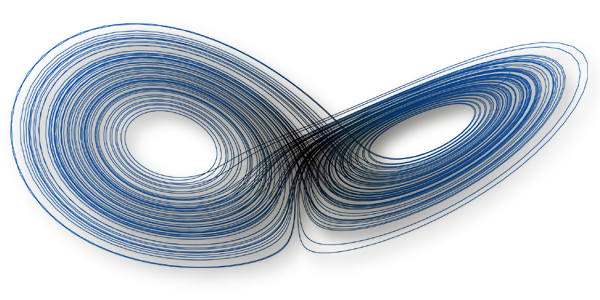
\includegraphics[width=.4\paperwidth]{cover.png}}

\date[unused]{ENSAM, Master 2, 2017--2018}

\begin{document}

\titleframe % Print the title as the first slide

%-------------------------------------------------------------------------------
%                           PRESENTATION SLIDES
%-------------------------------------------------------------------------------

\begin{frame}[t, c]{Overview from last time}{}
	\begin{itemize}
		\item In the previous lectures, we have solely considered dynamical systems of the form
		$$\dot{\mathbf{x}} = \mathbfcal{F}\left( \mathbf{x}, \mu \right),$$
		i.e.\ \emph{continuous-time} dynamical systems.

		\bigskip

		\item For such systems, you have seen how to :
		\begin{itemize}
			\item[$\hookrightarrow$] Compute fixed points, i.e.\ $\mathbfcal{F}\left( \mathbf{x} \right) = 0$.
			\item[$\hookrightarrow$] Determine their linear stability.
			\item[$\hookrightarrow$] Investigate how the dynamics in their vicinity are modified as we change $\mu$.
		\end{itemize}
	\end{itemize}

	\vspace{1cm}
\end{frame}

\begin{frame}[t, c]{What we will do in this lecture}{}
	\begin{itemize}
		\item In this lecture, we will see how to study systems like
		$$\mathbf{x}^{(k)} = \mathbfcal{G}\left( \mathbf{x}^{(k)}, \mu \right),$$
		i.e.\ \emph{discrete-time} dynamical systems.
	\end{itemize}

	\vspace{1cm}
\end{frame}

\begin{frame}[t, c]{}
	\centering
	\vspace{1cm}

	{\Large \textbf{Continuous vs.\ Discrete time}}

	\bigskip

	{\textgre{\textbf{What is time?}}}

\end{frame}

\begin{frame}[t, c]{Continuous time vs.\ Discrete time}{What is time?}
	\begin{columns}
		\begin{column}{.3\textwidth}
			\centering
			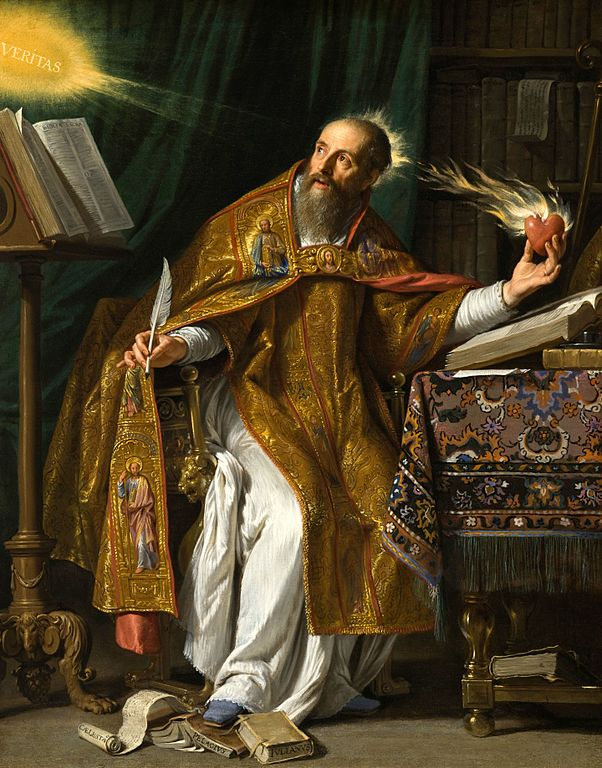
\includegraphics[width=.9\textwidth]{Saint_Augustin}
		\end{column}
		\begin{column}{.6\textwidth}
			\begin{quote}
				What, then, is time ? If no one asks me, I know what it is. If I wish to explain it to him who asks, I do not know.
			\end{quote}
			\begin{flushright}
				-- Saint Augustine of Hippo (354 -- 430).
			\end{flushright}
		\end{column}
	\end{columns}
\end{frame}

\begin{frame}[t, c]{Continuous time vs.\ Discrete time}{Zeno's dichotomy paradox}
	\centering
	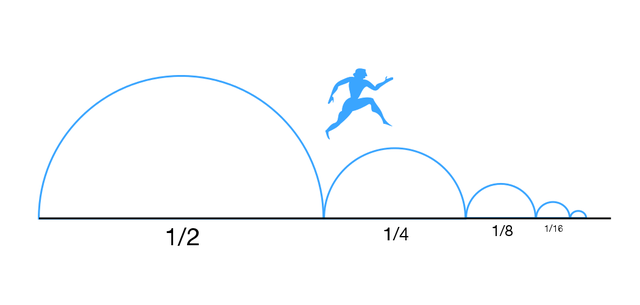
\includegraphics[width=.66\textwidth]{Zeno_Dichotomy_Paradox}

	\begin{quote}
		That which is in locomotion must arrive at the half-way stage before it arrives at the goal.
	\end{quote}
	\begin{flushright}
		-- As recounted by Aristotle.
	\end{flushright}

	\vspace{1cm}
\end{frame}

\begin{frame}[t, c]{Continuous time vs.\ Discrete time}{Why would a discrete model be super useful?}
	\centering

	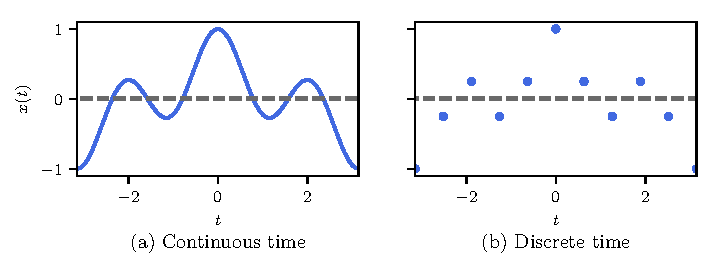
\includegraphics[width=.75\textwidth]{Continuous_vs_Discrete_bis}

	How to compute the mean $\bar{x}$?

	\begin{columns}
		\begin{column}{.4\textwidth}
			\centering
			$\bar{x} = \displaystyle \frac{1}{T} \int_{T_1}^{T_2} x(t)\ \mathrm{d}t$
		\end{column}
		\begin{column}{.4\textwidth}
			\centering
			$\bar{x} = \displaystyle \frac{1}{N} \sum_{n=0}^N x [n]$
		\end{column}
	\end{columns}
	\vspace{0.5cm}
\end{frame}

\begin{frame}[t, c]{Continuous time vs.\ Discrete time}{Can we really discretize time?}
	\centering

	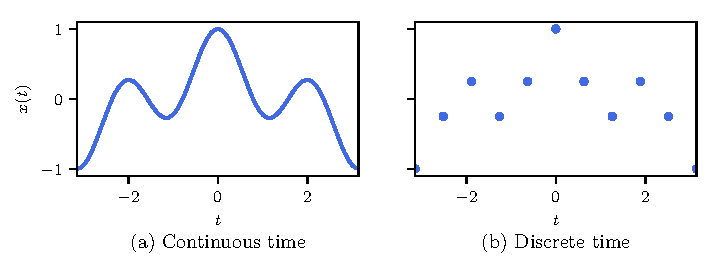
\includegraphics[width=.75\textwidth]{Continuous_vs_Discrete}

	How to make sure discretization does not cause loss of information?
\end{frame}

\begin{frame}[t, c]{Continuous time vs.\ Discrete time}{The Founding Fathers}
	\centering
	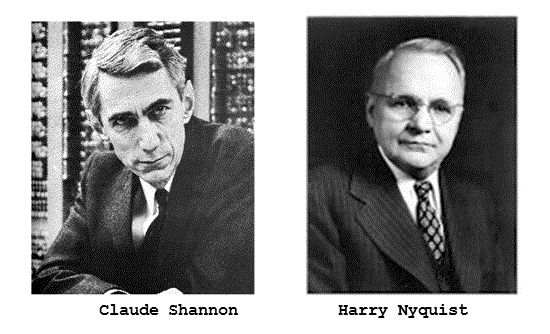
\includegraphics[height=.75\textheight]{Nyquist_Shannon}
\end{frame}

%-------------------------------------------------------------------------------
%                           SAMPLING THEOREM
%-------------------------------------------------------------------------------

\begin{frame}[t, c]{Continuous time vs.\ Discrete time}{The Sampling Theorem (1920)}

	Under appropriate "slowness" conditions for $x(t)$, we have:
	\begin{equation}
		x(t) = \sum_{n=-\infty}^{\infty} x \left[ n \right] \sinc \left( \displaystyle \frac{t - n T_s}{T_s} \right)
		\notag
	\end{equation}
	where $T_s$ is the \alert{\textbf{sampling period}} and $\displaystyle \sinc(x) = \frac{\sin(\pi x)}{\pi x}$ is the (normalized) \emph{cardinal sinus}.

\end{frame}

\begin{frame}[t, c]{Continuous time vs.\ Discrete time}{The Sampling Theorem (1920)}
	\centering
	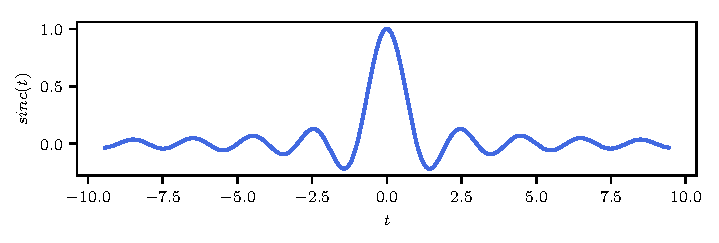
\includegraphics[width=.75\textwidth]{cardinal_sinus}
\end{frame}

\begin{frame}[t, c]{Continuous time vs.\ Discrete time}{The Sampling Theorem (1920)}
	\centering
	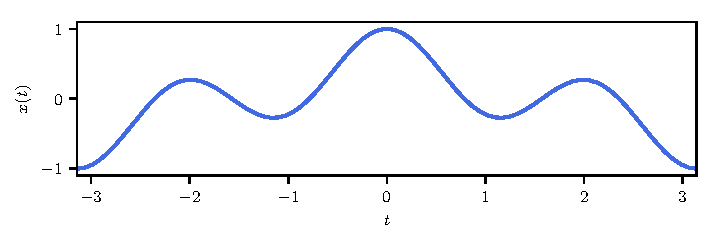
\includegraphics[width=.75\textwidth]{Sampling_theorem_a}
\end{frame}

\begin{frame}[t, c]{Continuous time vs.\ Discrete time}{The Sampling Theorem (1920)}
	\addtocounter{framenumber}{-1}
	\centering
	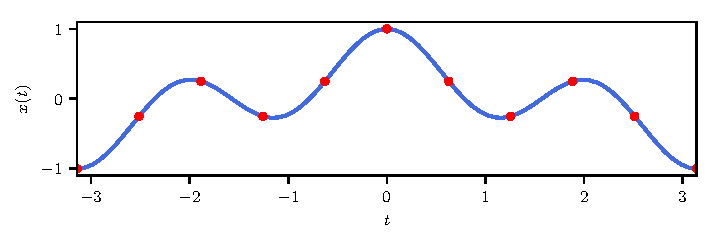
\includegraphics[width=.75\textwidth]{Sampling_theorem_b}
\end{frame}

\begin{frame}[t, c]{Continuous time vs.\ Discrete time}{The Sampling Theorem (1920)}
	\addtocounter{framenumber}{-1}
	\centering
	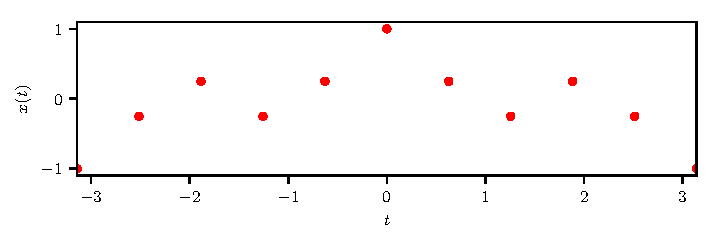
\includegraphics[width=.75\textwidth]{Sampling_theorem_c}
\end{frame}

\begin{frame}[t, c]{Continuous time vs.\ Discrete time}{The Sampling Theorem (1920)}
	\addtocounter{framenumber}{-1}
	\centering
	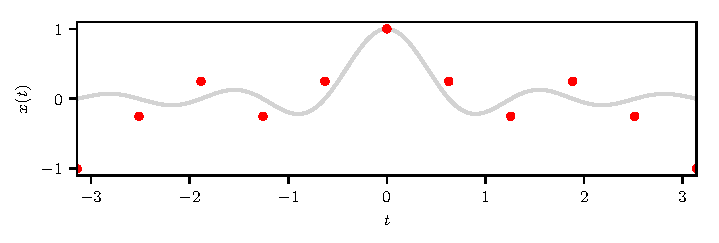
\includegraphics[width=.75\textwidth]{Sampling_theorem_d}
\end{frame}

\begin{frame}[t, c]{Continuous time vs.\ Discrete time}{The Sampling Theorem (1920)}
	\addtocounter{framenumber}{-1}
	\centering
	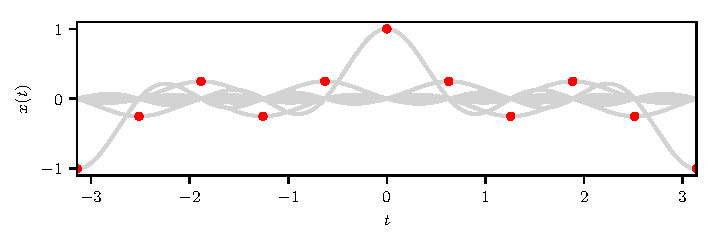
\includegraphics[width=.75\textwidth]{Sampling_theorem_e}
\end{frame}

\begin{frame}[t, c]{Continuous time vs.\ Discrete time}{The Sampling Theorem (1920)}
	\addtocounter{framenumber}{-1}
	\centering
	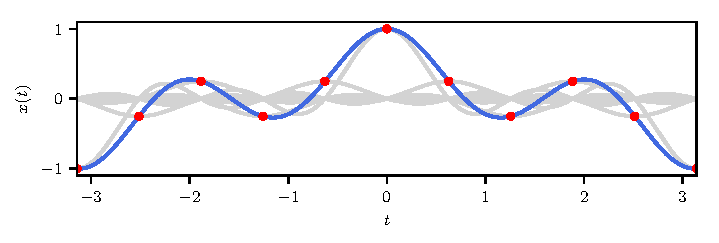
\includegraphics[width=.75\textwidth]{Sampling_theorem_f}
\end{frame}

\begin{frame}[t, c]{Continuous time vs.\ Discrete time}{The Sampling Theorem (1920)}
	\begin{itemize}
		\item The Sampling Theorem provides the connection between \emph{continuous} and \emph{discrete} time representations of the same signal.

		\bigskip

		\item From a practical point of view, it strongly relies on the choice of the sampling period $T_s$.
		\begin{itemize}
			\item[$\hookrightarrow$] This choice is guided by Fourier analysis.
		\end{itemize}
	\end{itemize}
	\vspace{1cm}
\end{frame}

\begin{frame}[t, c]{}
	\centering
	\vspace{1cm}

	{\Large \textbf{Discrete-time dynamical systems}}

	\bigskip

	{\textgre{\textbf{Example: the logistic map}}}

\end{frame}

\begin{frame}[t, c]{Logistic map}{Overview}
	\begin{itemize}
		\item The \alert{\textbf{logistic map}} is a quadratic polynomial mapping given by
		$$x_{k+1} = \mu x_k ( 1 - x_k),$$
		where $x_k \in \left[ 0, 1 \right]$ is the ratio of existing population to the maximum possible population, and $\mu \in \left[ 0 , 4 \right]$.

		\bigskip

		\item This nonlinear difference equation capture two effects:
		\begin{enumerate}
			\item \emph{reproduction}, i.e.\ population increases if $x$ is small.
			\item \emph{starvation}, i.e.\ individuals die due to the limited carrying capacity.
		\end{enumerate}
	\end{itemize}

	\vspace{1cm}
\end{frame}

\begin{frame}[t, c]{Logistic map}{Fixed point}
	\begin{itemize}
		\item Fixed points of a discrete-time dynamical systems are given by
		$$\mathbf{x}^* = \mathbfcal{G} \left( \mathbf{x}^* \right).$$

		\bigskip

		\item For the present system, this can be visualized graphically.
	\end{itemize}

	\vspace{1cm}
\end{frame}

\begin{frame}[t, c]{Logistic map}{Fixed points}
	\centering
	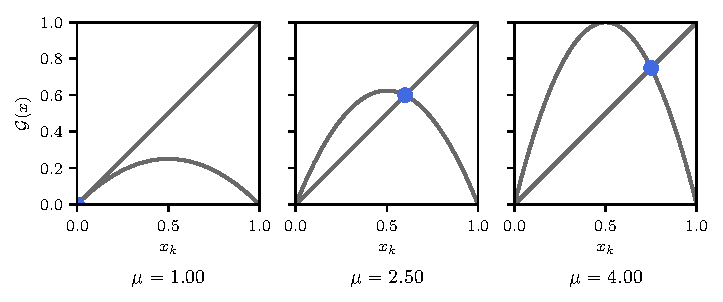
\includegraphics[width=.75\textwidth]{logistic_map_fixed_points}

	\vspace{1cm}
\end{frame}

\begin{frame}[t, c]{Logistic map}{Cobweb and phase plane for $\mu = 1$}
	\begin{minipage}{.48\textwidth}
		\centering
		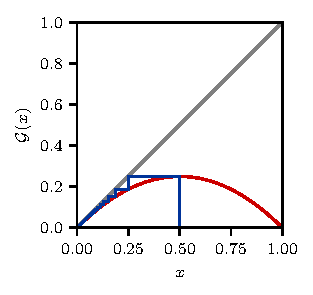
\includegraphics[width=.75\textwidth]{logistic_map_cobweb_plot_0}
	\end{minipage}%
	\begin{minipage}{.48\textwidth}
		\centering
		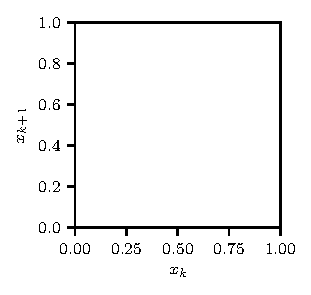
\includegraphics[width=.75\textwidth]{logistic_map_phase_plane_0}
	\end{minipage}

	\vspace{1cm}
\end{frame}

\begin{frame}[t, c]{Logistic map}{Cobweb and phase plane for $\mu = 1.32$}
	\begin{minipage}{.48\textwidth}
		\centering
		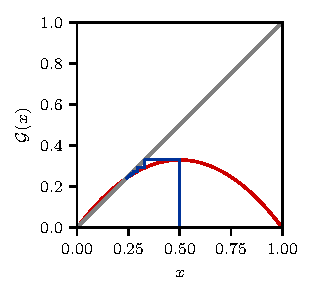
\includegraphics[width=.75\textwidth]{logistic_map_cobweb_plot_1}
	\end{minipage}%
	\begin{minipage}{.48\textwidth}
		\centering
		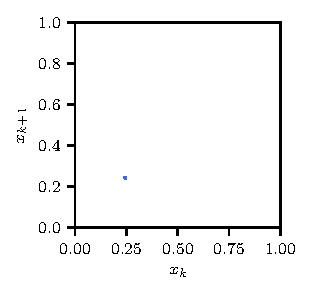
\includegraphics[width=.75\textwidth]{logistic_map_phase_plane_1}
	\end{minipage}

	\vspace{1cm}
\end{frame}

\begin{frame}[t, c]{Logistic map}{Cobweb and phase plane for $\mu = 1.64$}
	\begin{minipage}{.48\textwidth}
		\centering
		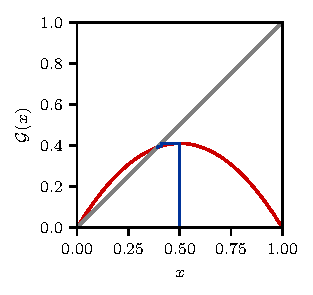
\includegraphics[width=.75\textwidth]{logistic_map_cobweb_plot_2}
	\end{minipage}%
	\begin{minipage}{.48\textwidth}
		\centering
		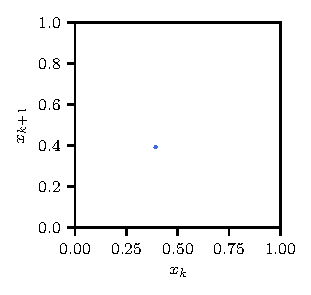
\includegraphics[width=.75\textwidth]{logistic_map_phase_plane_2}
	\end{minipage}

	\vspace{1cm}
\end{frame}

\begin{frame}[t, c]{Logistic map}{Cobweb and phase plane for $\mu = 1.96$}
	\begin{minipage}{.48\textwidth}
		\centering
		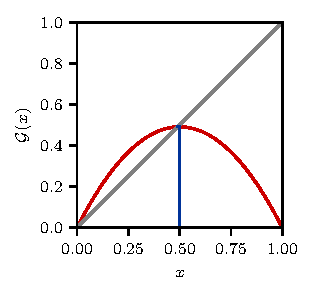
\includegraphics[width=.75\textwidth]{logistic_map_cobweb_plot_3}
	\end{minipage}%
	\begin{minipage}{.48\textwidth}
		\centering
		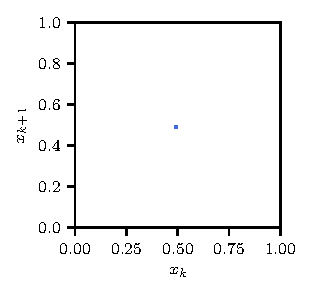
\includegraphics[width=.75\textwidth]{logistic_map_phase_plane_3}
	\end{minipage}

	\vspace{1cm}
\end{frame}

\begin{frame}[t, c]{Logistic map}{Cobweb and phase plane for $\mu = 2.28$}
	\begin{minipage}{.48\textwidth}
		\centering
		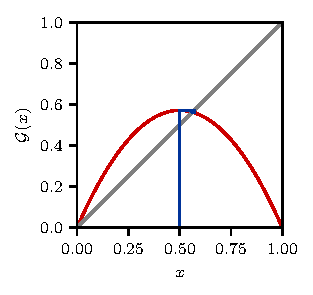
\includegraphics[width=.75\textwidth]{logistic_map_cobweb_plot_4}
	\end{minipage}%
	\begin{minipage}{.48\textwidth}
		\centering
		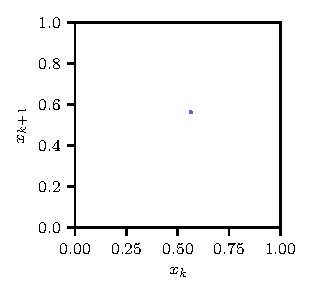
\includegraphics[width=.75\textwidth]{logistic_map_phase_plane_4}
	\end{minipage}

	\vspace{1cm}
\end{frame}

\begin{frame}[t, c]{Logistic map}{Cobweb and phase plane for $\mu = 2.61$}
	\begin{minipage}{.48\textwidth}
		\centering
		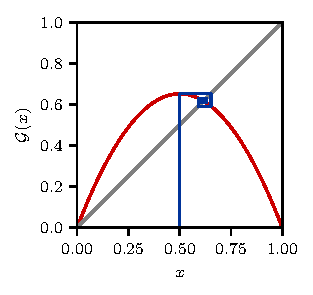
\includegraphics[width=.75\textwidth]{logistic_map_cobweb_plot_5}
	\end{minipage}%
	\begin{minipage}{.48\textwidth}
		\centering
		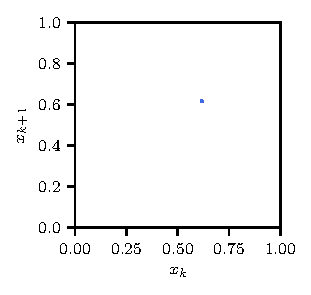
\includegraphics[width=.75\textwidth]{logistic_map_phase_plane_5}
	\end{minipage}

	\vspace{1cm}
\end{frame}

\begin{frame}[t, c]{Logistic map}{Cobweb and phase plane for $\mu = 2.93$}
	\begin{minipage}{.48\textwidth}
		\centering
		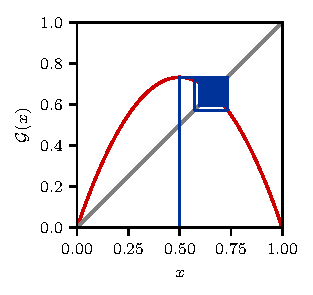
\includegraphics[width=.75\textwidth]{logistic_map_cobweb_plot_6}
	\end{minipage}%
	\begin{minipage}{.48\textwidth}
		\centering
		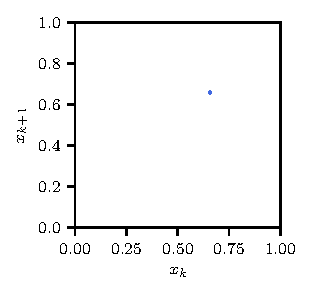
\includegraphics[width=.75\textwidth]{logistic_map_phase_plane_6}
	\end{minipage}

	\vspace{1cm}
\end{frame}

\begin{frame}[t, c]{Logistic map}{Cobweb and phase plane for $\mu = 3.25$}
	\begin{minipage}{.48\textwidth}
		\centering
		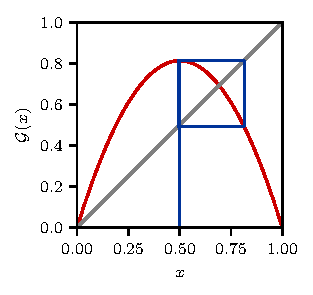
\includegraphics[width=.75\textwidth]{logistic_map_cobweb_plot_7}
	\end{minipage}%
	\begin{minipage}{.48\textwidth}
		\centering
		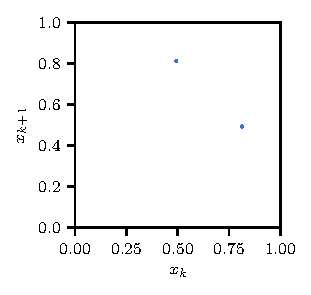
\includegraphics[width=.75\textwidth]{logistic_map_phase_plane_7}
	\end{minipage}

	\vspace{1cm}
\end{frame}

\begin{frame}[t, c]{Logistic map}{Cobweb and phase plane for $\mu = 3.57$}
	\begin{minipage}{.48\textwidth}
		\centering
		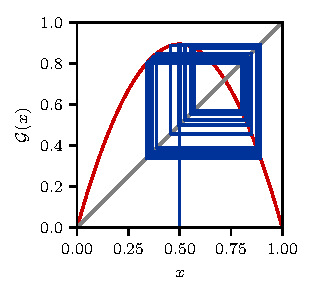
\includegraphics[width=.75\textwidth]{logistic_map_cobweb_plot_8}
	\end{minipage}%
	\begin{minipage}{.48\textwidth}
		\centering
		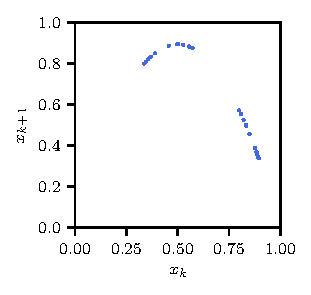
\includegraphics[width=.75\textwidth]{logistic_map_phase_plane_8}
	\end{minipage}

	\vspace{1cm}
\end{frame}

\begin{frame}[t, c]{Logistic map}{Cobweb and phase plane for $\mu = 3.9$}
	\begin{minipage}{.48\textwidth}
		\centering
		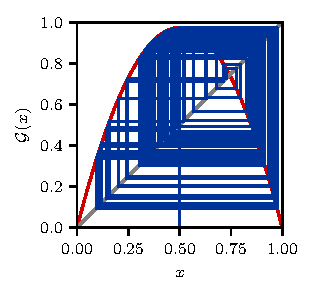
\includegraphics[width=.75\textwidth]{logistic_map_cobweb_plot_9}
	\end{minipage}%
	\begin{minipage}{.48\textwidth}
		\centering
		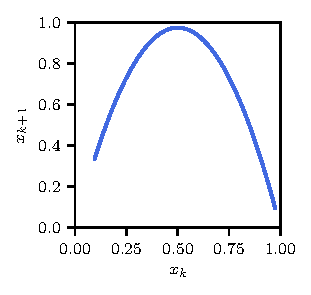
\includegraphics[width=.75\textwidth]{logistic_map_phase_plane_9}
	\end{minipage}

	\vspace{1cm}
\end{frame}

\begin{frame}[t, c]{Logistic map}{Chaos vs.\ Randomness}
	\centering
	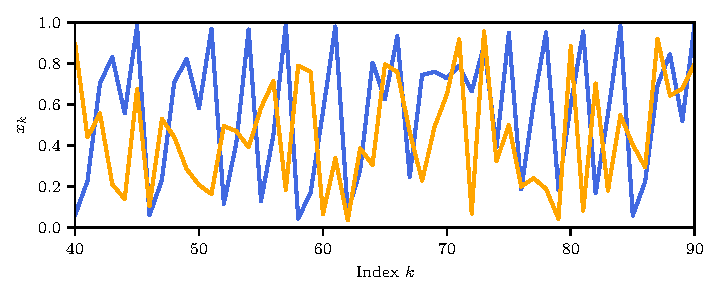
\includegraphics[width=.75\textwidth]{chaos_vs_randomness}

	\vspace{1cm}
\end{frame}

\begin{frame}[t, c]{Logistic map}{Chaos vs.\ Randomness}
	\begin{minipage}{.48\textwidth}
		\centering
		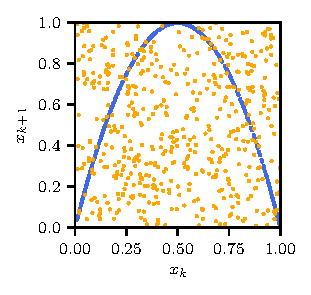
\includegraphics[width=.75\textwidth]{chaos_vs_randomness_phase_plane}
	\end{minipage}%
	\hfill
	\begin{minipage}{.48\textwidth}
		\begin{itemize}
			\item Chaotic dynamics $\neq$ Random dynamics.

			\medskip

			\item No pattern in random dynamics vs.\ so-called \emph{strange attractors} in chaotic dynamics.
		\end{itemize}
	\end{minipage}

	\vspace{1cm}
\end{frame}

\begin{frame}[t, c]{Logistic map}{Bifurcation diagram}
	\centering
	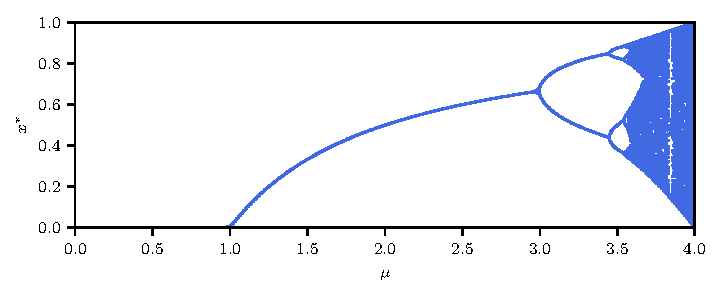
\includegraphics[width=.75\textwidth]{logistic_map_bifurcation_overview}

	\vspace{1cm}
\end{frame}

\begin{frame}[t, c]{Logistic map}{Bifurcation diagram}
	\centering
	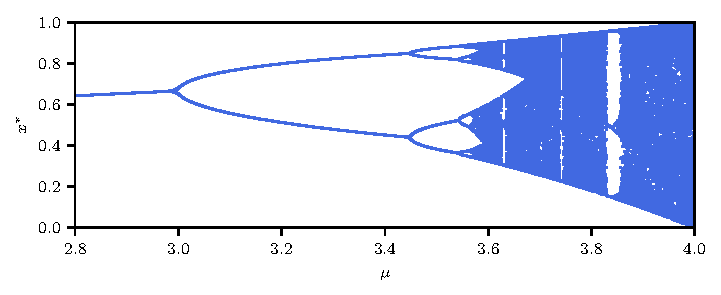
\includegraphics[width=.75\textwidth]{logistic_map_bifurcation_zoom_1}

	\vspace{1cm}
\end{frame}

\begin{frame}[t, c]{Logistic map}{Bifurcation diagram}
	\centering
	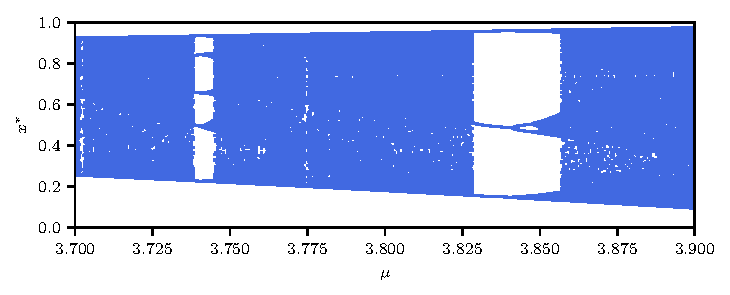
\includegraphics[width=.75\textwidth]{logistic_map_bifurcation_zoom_2}

	\vspace{1cm}
\end{frame}

\begin{frame}[t, c]{Logistic map}{Bifurcation diagram}
	\centering
	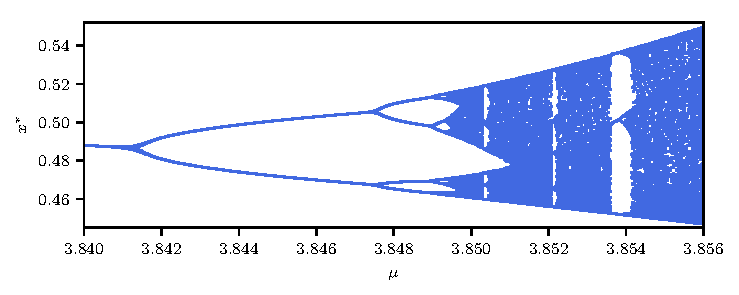
\includegraphics[width=.75\textwidth]{logistic_map_bifurcation_zoom_3}

	\vspace{1cm}
\end{frame}

\begin{frame}[t, c]{}
	\centering
	\vspace{1cm}

	{\Large \textbf{Discrete-time dynamical systems}}

	\bigskip

	{\textgre{\textbf{Let's be more formal.}}}

\end{frame}

\begin{frame}[t, c]{Linear systems}{Continuous time vs.\ Discrete time}
	\begin{itemize}
		\item A similar connection exists between continuous time and discrete time representations of \alert{\textbf{Linear Time Invariant}} (LTI) \alert{\textbf{Dynamical Systems}}.

		\bigskip

		\item Working in one representation or the other may simplify certain calculations that would otherwise be complicated.
	\end{itemize}
	\vspace{1cm}
\end{frame}

\begin{frame}[t, c]{Linear systems}{Continuous time vs.\ Discrete time}
	\begin{minipage}{.48\textwidth}
		\begin{itemize}
			\item Let us consider the following LTI dynamical system
			\begin{equation}
				\displaystyle \frac{\mathrm{d}x}{\mathrm{d}t} = -k x.
				\notag
			\end{equation}

			\bigskip

			\item Its solution is given by
			\begin{equation}
				x(t) = e^{-k t}x_0
				\notag
			\end{equation}
		\end{itemize}
		\vspace{.5cm}
	\end{minipage}%
	\hfill
	\begin{minipage}{.48\textwidth}
		\centering
		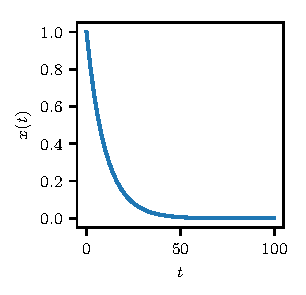
\includegraphics[width=.75\textwidth]{first_order_system}
	\end{minipage}
\end{frame}

\begin{frame}[t, c]{Linear systems}{Continuous time vs.\ Discrete time}
	\begin{minipage}{.48\textwidth}
		\begin{itemize}
			\item For a given sampling period $T_s$, the discrete time counterpart of the previous system is
			\begin{equation}
				\displaystyle x[i] = \alpha x[i-1]
				\notag
			\end{equation}
			with $\alpha = e^{-k T_s}$.

			\bigskip

			\item This is known as a first-order \alert{\textbf{Auto-Regressive}} (AR1) model.
			\end{itemize}
		\vspace{1.25cm}
	\end{minipage}%
	\hfill
	\begin{minipage}{.48\textwidth}
		\centering
		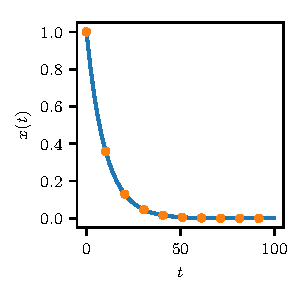
\includegraphics[width=.75\textwidth]{first_order_system_bis}
	\end{minipage}
\end{frame}

\begin{frame}[t, c]{Linear systems}{Continuous time vs.\ Discrete time}
	\centering
	\begin{itemize}
		\item Let us consider the following LTI dynamical system
		\begin{equation}
			\ddot{x} = -2k \dot{x} - \omega_0^2 x
			\notag
		\end{equation}
	\end{itemize}
	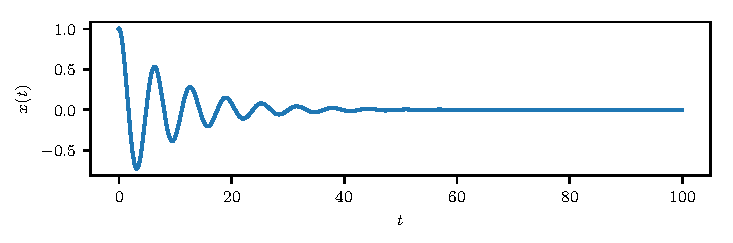
\includegraphics[width=.75\textwidth]{second_order_system}
\end{frame}

\begin{frame}[t, c]{Linear systems}{Continuous time vs.\ Discrete time}
	\centering
	\begin{itemize}
		\item Its discrete time counterpart is an AR2 model given by
		\begin{equation}
			x[i] = \alpha_1 x[i-1] + \alpha_2 x[i-2]
			\notag
		\end{equation}
	\end{itemize}
	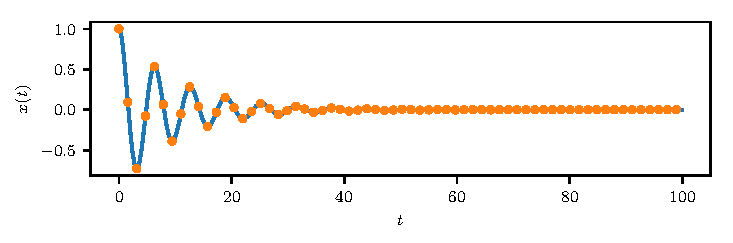
\includegraphics[width=.75\textwidth]{second_order_system_bis}
\end{frame}

\begin{frame}{Linear systems}{Continuous time \textbf{to} Discrete time}
	\begin{itemize}
		\item The solution to a continuous time linear dynamical system is given by
		$$\mathbf{x}(t) = \exp \left( \mathbfcal{A} t \right) \textbf{x}_0.$$

		\item If it is sampled at a period $T$, one gets the sequence :
		$$\left\{ \mathbf{x}(0) , \mathbf{x}(T), \mathbf{x}(2T) , \cdots, \mathbf{x}(kT) \right\}$$

		\item From a discrete-time point of view, this sequence can be modeled as
		$$ \mathbf{x}_{k+1} = \underbrace{\exp \left( \mathbfcal{A} T \right) }_{\mathbfcal{M}} \mathbf{x}_k$$
	\end{itemize}
\end{frame}

\begin{frame}[t, c]{Discrete-time linear systems}{Linear stability}
	\begin{itemize}
		\item Given a discrete-time linear system
		$$\mathbf{x}_{k+1} = \mathbfcal{M} \mathbf{x}_k,$$
		one can write
		$$\mathbf{x}_{k+1} = \mathbfcal{M}^{k} \mathbf{x}_0.$$

		\bigskip

		\item Its stability is thus determined by the eigenvalues of $\mathbfcal{M}$.
		\begin{itemize}
			\item[$\hookrightarrow$] If $\vert \lambda_1 \vert > 1$, the system is linearly unstable.
			\item[$\hookrightarrow$] If $\vert \lambda_1 \vert < 1$, the system is linearly stable.
		\end{itemize}
	\end{itemize}

	\vspace{1cm}
\end{frame}

\begin{frame}[t, c]{Discrete-time systems}{Exercise}
	Consider the logistic map
	$$ x_{k+1} = \mu x_k ( 1 - x_k )$$
	and do the following:
	\begin{enumerate}
		\item Find its fixed points as a function of $\mu$.
		\item Study their linear stability.
	\end{enumerate}

	\bigskip

	\underline{If you have your computer}:
	\begin{enumerate}
		\item Given $f(x) = \mu x ( 1 - x )$, try to find the fixed points of
		$$x_{k+2} = f \left( f\left( x_k \right) \right).$$
		\item Study their linear stability.
	\end{enumerate}

	\vspace{1cm}
\end{frame}

\end{document}
